% ==============================================================================
\section{Prototipo físico}
\label{sec:dev_prototipo}
% ==============================================================================

El armazón de los lentes se diseñó en un modelador CAD. Los sensores definidos en la
sección de electrónica de TT1 van alojados en un frente ensanchado, por encima de los
cristales, y las patillas son anchas para dar espacio al cableado. La
Figura~\ref{fig:proto_explosivo} muestra la vista explosionada. La Camera Module 3 Wide
va en el centro del frente, a la altura del puente de la nariz, de modo que queda
alineada con la dirección en la que mira el usuario; el módulo de visión y el cálculo de
distancias por plano de piso parten de esa suposición. Los dos sensores ultrasónicos
MB1232 van en el frente, uno sobre cada cristal, y la IMU BNO055 va plana en la parte
superior del mismo frente. El resto de las tarjetas se aloja detrás de la cámara y en la
patilla derecha, donde queda un conector accesible desde el exterior.

\begin{figure}[H]
    \centering
    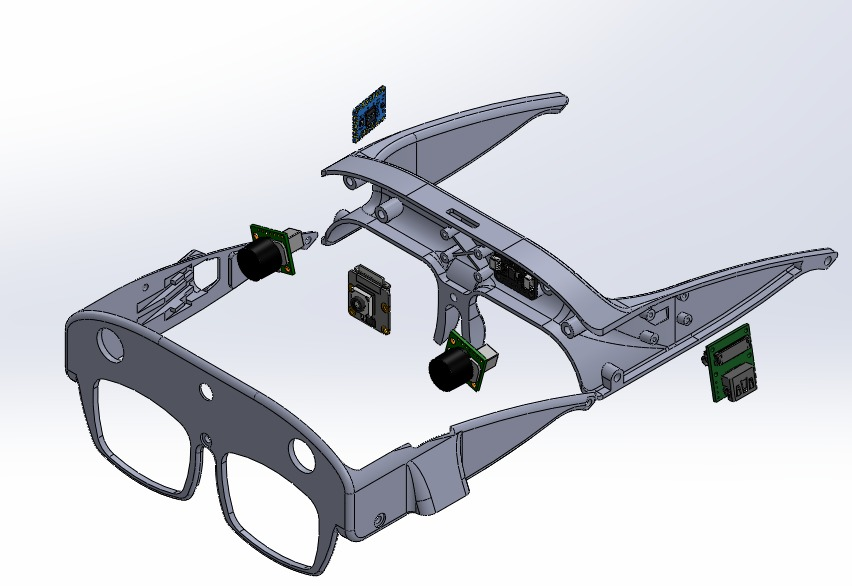
\includegraphics[width=0.85\textwidth]{Capturas_TT2/hardware/Render.jpeg}
    \caption{Vista explosionada del armazón, con la cámara al centro y los sensores
    ultrasónicos sobre cada cristal.}
    \label{fig:proto_explosivo}
\end{figure}

Las Figuras~\ref{fig:proto_transparente} y \ref{fig:proto_armado} muestran el diseño
armado, primero con el frente transparente para ver la disposición interna y después
con el acabado final.

\begin{figure}[H]
    \centering
    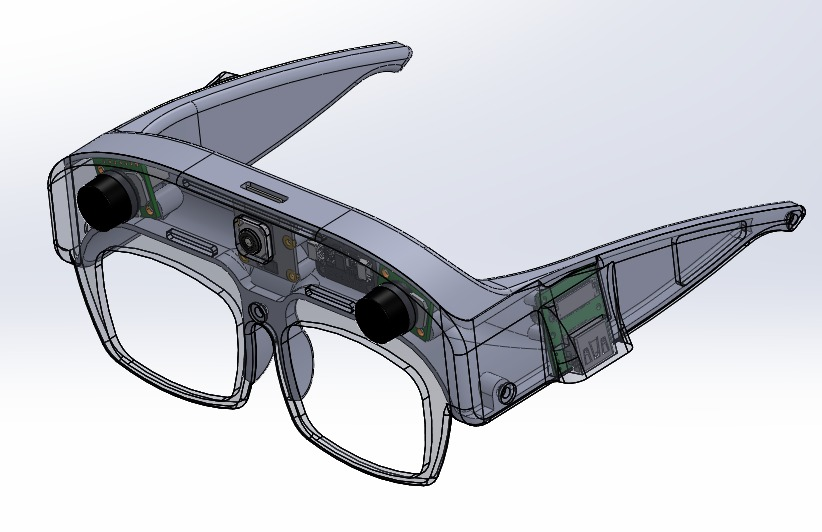
\includegraphics[width=0.8\textwidth]{Capturas_TT2/hardware/VistaPrincipal.jpeg}
    \caption{Diseño armado con el frente transparente.}
    \label{fig:proto_transparente}
\end{figure}

\begin{figure}[H]
    \centering
    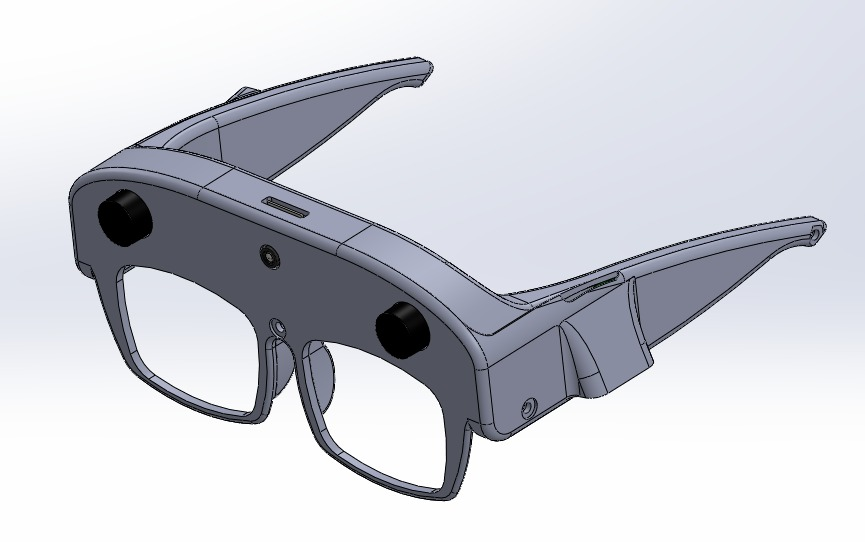
\includegraphics[width=0.8\textwidth]{Capturas_TT2/hardware/VistaReal.jpeg}
    \caption{Diseño armado con el acabado final.}
    \label{fig:proto_armado}
\end{figure}

\TODO{agregar fotos del prototipo fabricado y armado, y describir el material, el
método de fabricación, el peso final y dónde van la Raspberry Pi y la batería}.

Los dos ultrasónicos apuntan hacia adelante, en la misma dirección que la cámara, y
están separados unos 10~cm. Como los sensores y la IMU van en el mismo frente rígido, el
cabeceo que mide la IMU es también el de la cámara y el de los ultrasónicos. Toda esta
geometría se concentra en un solo archivo, \texttt{montaje.py}, que usan el driver de
los sensores, la fusión, las alertas y el simulador, y que se ajusta con las medidas
tomadas sobre el prototipo.

En TT1 se había planteado que los ultrasónicos cubrieran los costados del usuario. Al
revisar la hoja de datos se vio que el MB1232 tiene un haz angosto, de unos
$\pm 14^\circ$, así que sirve poco para vigilar los lados. Puesto al frente, en cambio,
su haz coincide con lo que ve la cámara. Eso permite confirmar o descartar las
detecciones visuales, avisar de vidrios y mamparas que la cámara no reconoce y corregir
el estado de las puertas, como se explica en las secciones de SLAM, visión y alertas.
El costo de esta decisión es que los costados quedan cubiertos solo por la cámara y que
el mapa registra menos superficie lateral (Tabla~\ref{tab:mapeo_us}).
